\chapter[Introduction]{Introduction}

\section[Recent developments in High Energy Physics]{Recent developments in High Energy Physics}

The Standard Model (SM) of Particle Physics \cite{Standard-model} is the most successful theory for describing our universe at the smallest scales. It describes natural phenomena such as interactions of particles that constitute building blocks of matter as we know it.

The subatomic particles can be organised in two families. The first is composed of fermions, particles with half-integer spin that constitute matter (Table \ref{tab:Fermions}). Two types of fermions exist: quarks (bearing a charge $+2/3$~e or $-1/3$~e, where e is the elementary charge unit), and leptons, featuring a charge of $-1$~e (charged leptons) or $0$ (neutrinos). Furthermore fermions are also grouped in three generations with increasing mass. The second family of particles is composed of bosons, particles of integer spin that mediate the interactions between fermions (Table \ref{tab:Bosons}). The Standard Model assigns to each fermion a corresponding anti-particle, identical but featuring the opposite charge.

\begin{table}[!b]
  \centering
    \begin{tabular}{l c c c}
    \toprule
    Generation  & I & II  & III \\
    \midrule
    Quarks  & Up  & Charm & Top \\
              & Down& Strange & Bottom \\
    \hline
    Leptons		& Electron & Muon & Tau	\\
              & Electron neutrino & Muon neutrino & Tau neutrino	\\
    \bottomrule
    \end{tabular}
  \caption{Particles composing the fermion family.} \label{tab:Fermions}
\end{table}


Matter is normally formed of first generation fermions, e.g.\ electrons, and compounds of quarks, e.g.\ protons and neutrons. The aggregates of particles can be mesons (pairs of one quark and one anti-quark) or baryons (a triplet of quarks). For example, a proton is a baryon formed of two up quarks and one down quark, while a neutron is a baryon formed of one up quark up and two down quarks. More exotic  combinations have been observed in recent years, e.g. at the LHCb experiment at CERN \cite{LHCb:tetraquark,LHCb:pentaquark, LHCb:pentaquark2}. Interactions between subatomic particles are mediated by the exchange of bosons, particles of integer spin. Quarks forming baryons are held together by the strong force, mediated by gluons. They also interact via the weak force, mediated by the $W^\pm$ and $Z^0$ bosons and the electromagnetic force, mediated by photons. Charged leptons interact only via the weak and electromagnetic forces. The electromagnetic force binds nuclei and electrons, forming atoms and then molecules, shaping matter as we perceive it. Neutrinos interact only via the weak force. The final component is the Higgs field, mediated by the Higgs boson, which gives mass to all the other particles \cite{PhysRevLett.13.508}. A particle associated with the Higgs field was observed in 2012 at the Large Hadron Collider (LHC) \cite{LHC:cdr} by the ATLAS and CMS experiments  \cite{ATLAS:Higgs, CMS:Higgs}.

\begin{table}[!t]
  \centering
    \begin{tabular}{l c }
    \toprule
    Boson & Function\\
    \midrule
    Photon                    & Electromagnetic interaction\\
    $W^\pm$ and $Z^0$ bosons  & Weak interaction\\
    Gluon                     & Strong interaction\\
    Higgs boson $H^0$         & Higgs field mediator\\
    \bottomrule
    \end{tabular}
  \caption{Particles comprising the boson family.} \label{tab:Bosons}
\end{table}

Although the Standard Model is a remarkable achievement of humanity in the understanding of particle physics, a number of questions remain unaddressed and cannot be explained with the present theory, even after the observation of the Higgs boson, e.g.\ a phenomenon known as neutrino oscillation, leading to the change of flavour of such a particle \cite{nobel-neutrino-osc}. Furthermore, the SM does not include the gravitational force, and it does not include the dark matter and dark energy that were proposed to explain some cosmological observations \cite{RevModPhys.75.559}. Moreover, the SM does not explain why the universe is observed as predominantly made of matter, while the creation of equal amounts of matter and antimatter in the Big Bang would be expected, as the forces of nature are predominantly symmetrical between them.

To answer these and other questions, a number of theories have been developed, some of which propose new particles that have not yet been observed in particle colliders. The search for these new particles, together with the study of the properties of the recently discovered Higgs boson, calls for a new generation of high energy particle colliders.


\section[Particle colliders]{Particle colliders}

The vast majority of the discoveries in particle physics were produced using particle beam colliders. They allow physicists to perform experiments in controlled conditions, which is much harder to achieve when observing particles in nature, e.g. observing the interaction of cosmic rays with the atmosphere from space~\cite{Adams:2014xuv} or from the ground~\cite{ThePierreAuger:2015rma}. A particle collider consists of a particle accelerator in which two particle beams are accelerated and collided with each other head-on. The products of the collisions are recorded and studied, in order to obtain an insight into the physical processes that take place. The observation rate R of a given physical process X arising from the interaction between the colliding particles is

\begin{equation}
R(X) = \mathscr{L}\sigma(X)\label{eq:rate}
\end{equation}
where $\sigma(X)$ is the cross section representing the probability of the process X happening, which includes the collision energy dependence, and $\mathscr{L}$ is the luminosity, which depends on the particle beam parameters. The luminosity can be expressed as

\begin{equation}
\mathscr{L} = \frac{1}{4\pi} \frac{N_1 N_2 f n_b}{\sigma_x \sigma_y} H
\end{equation}
where $N_{1,2}$ is the number of particles in one of the colliding bunches, $f$ is the collision frequency, $n_b$ is the number of colliding bunches per cycle, $\sigma_x$ and $\sigma_y$ are the transverse beam dimensions, and $H$ is a correction factor for luminosity enhancement or depression, e.g. due to beam-beam effects, non-head-on collisions, such as bunch crossing at an angle or off-centre, or the hourglass effect~\cite{handbook_acc_phys}. 

For a given energy, the cross section is a constant number, while the luminosity depends on the beam parameters. In order to study rare processes, i.e. those with a low cross section, it is then necessary to increase the luminosity as much as possible. The luminosity and collision energy increase are ultimately limited by numerous technical factors, which vary for each accelerator type and are outlined in the next section.



\section[Limitations for future colliders]{Limitations for future colliders}
Pursuing the search for particles at higher collision energies requires a new generation of particle accelerators. Particle colliders have improved over the past 60 years, reaching unprecedented levels of technical development. Devising a new generation of accelerators requires many technical limitations \cite{CAS:Ferrario-limitiations, CAS:Assman-limitiations} to be overcome and the exploitation of refined engineering solutions. A number of accelerator types were studied to overcome these obstacles. They are presented below together with their main limitations:

\begin{itemize}
\item \textbf{Circular hadron colliders:} the development of high energy circular hadron colliders is mainly limited by the required size and the availability of strong magnets. In fact, the particle momentum in a circular collider is 
\begin{equation}
p = e\rho B \label{eq:lim1}
\end{equation}
where $e$ is the elementary charge, $\rho$ is the accelerator radius, and $B$ is the dipole magnetic field. Consequently, an increased beam momentum (and energy) requires a larger radius or a stronger magnetic field. Presently, the LHC dipoles reach a field of 8.33~T. Stronger magnets are being designed and tested for the LHC High Luminosity Upgrade (HL-LHC) \cite{HL-LHC:cdr}. However, they have not yet demonstrated a sufficient performance to be installed in an operational accelerator \cite{Rossi:IPAC19}. If the high-field magnet technology is successful, it has been proposed to double the LHC energy in the so called High Energy LHC (HE-LHC) \cite{HE-LHC:cdr}. Additionally, the Future Circular Collider (FCC)~\cite{FCC-hh:cdr} project has been proposed to increase the accelerator circumference to 80-100~km while using high-field magnets, aiming for 100~TeV collision energy.
\item \textbf{Circular lepton colliders:} circular lepton accelerators not only have to obey the limitation of Equation~\ref{eq:lim1}, but they are also principally limited by the emission of synchrotron radiation. The mean power radiated by bending a particle beam trajectory into a circle is given by
\begin{equation}
P\propto \frac{1}{\rho^2} \frac{E^4}{m_0^4}
\end{equation}
where $m_0$ is the rest mass of the particle and $E$ is the particle beam energy \cite{JAS:synchro-radiation, JOHNSON199723}. The amount of radiated power has been a massive limitation in the past, e.g. the electron beam in the 27~km LEP2 ring \cite{LEP2:cdr} at the top energy of $104.5$~GeV  lost more than $3$~GeV of energy per revolution. Any equipment installed in a circular lepton accelerator must sustain constant exposure to large amounts of radiation. The use of muons instead of electrons has been proposed due to their larger mass, however muon beams are limited by their short lifetime. The production of a sufficiently intense muon beam and its acceleration to the energy required for the experiments, within the time limitations imposed by the decay, is challenging~\cite{Rubbia:summary}. Due to the additional complications, solutions to many of the technical problems are being researched in a number of institutions \cite{Wang_2016, BONESINI2013203, Antonelli:2015nla}. As an alternative, the FCC study has proposed to install an electron-positron collider in the 100~km tunnel (FCC-ee) \cite{FCC-ee:cdr}, profiting from the large ring radius to reduce the radiated power.
\item \textbf{Linear electron colliders:} the particle momentum in a linear collider is $$p \propto L \, G_\text{acc}$$ where $L$ is the total accelerating length and $G_\text{acc}$ is the accelerating gradient per unit length. Many designs have been proposed for linear electron-positron colliders, ranging from more traditional to the most exotic technologies. The International Linear Collider (ILC) \cite{ILC:cdr} proposed an accelerator based on superconducting radiofrequency (RF) cavities. The Compact Linear Collider (CLIC) \cite{CLIC:cdr} is based on normal-conducting high-gradient RF technology and a novel two-beam acceleration scheme in order to reach a high beam energy while minimising the accelerator length. Ultimately, any acceleration technology relying on RF cavities is limited by the surface electrical breakdown \cite{KilpLimit}. To overcome this limitation, a  number of innovative techniques relying on plasma are under study. So far none of them appear credible for an operational collider due to the required high beam brightness \cite{doi:10.1142/S1793626816300097}, even though record accelerating gradients were reached \cite{Blumenfeld:2007ph}. Innovative acceleration techniques are reviewed in Section~\ref{sec:two_beam_tech}.
\end{itemize}

The footprint of the CLIC and FCC projects compared to the existing LHC is shown in Fig.~\ref{fig:FCC_vs_LHC}. LEP2 and the LHC were designed to fit in the same 27~km long tunnel, as well as the HL-LHC and HE-LHC projects. Regarding linear colliders, both the ILC (see Fig.~\ref{fig:ILC_schematic}) and CLIC project (see Fig.~\ref{fig:CLIC_schematic}) foresee long footprints of the order of  50~km length for the top energy versions, although shorter designs are considered for the lower energy versions.


% \begin{figure}[!h]
% \centering
% 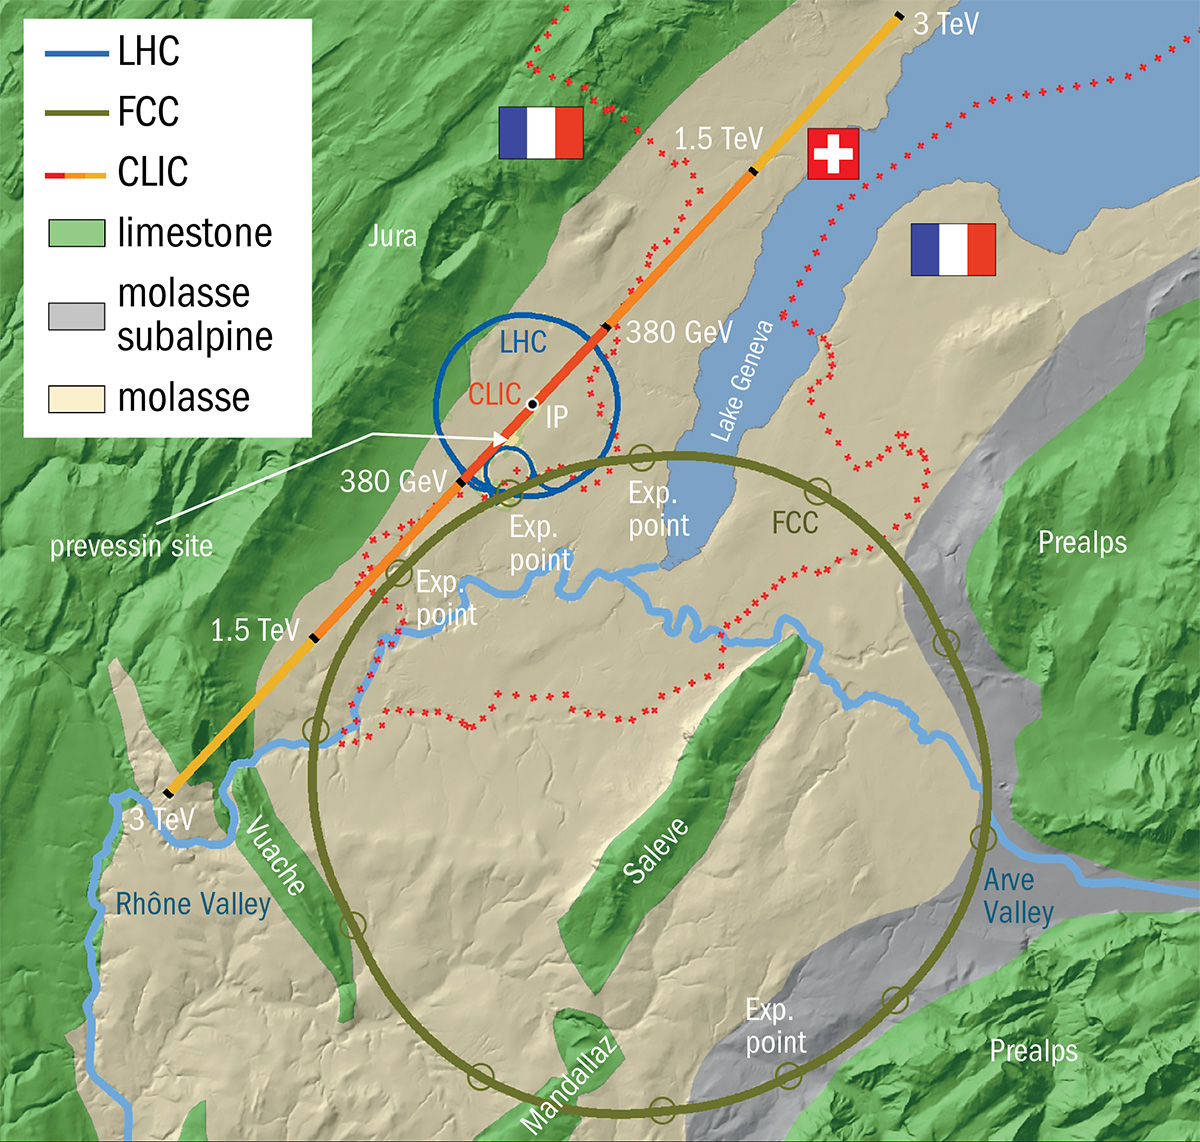
\includegraphics[width=120mm, keepaspectratio]{pictures/FCC_vs_CLIC_vs_LHC}
% \caption{Dimension comparison of the CLIC and FCC project with the existing LHC accelerator in the Geneva area \cite{CERN-COURIER-59-5}.}
% \label{fig:FCC_vs_LHC}


% \vspace{5mm}
% 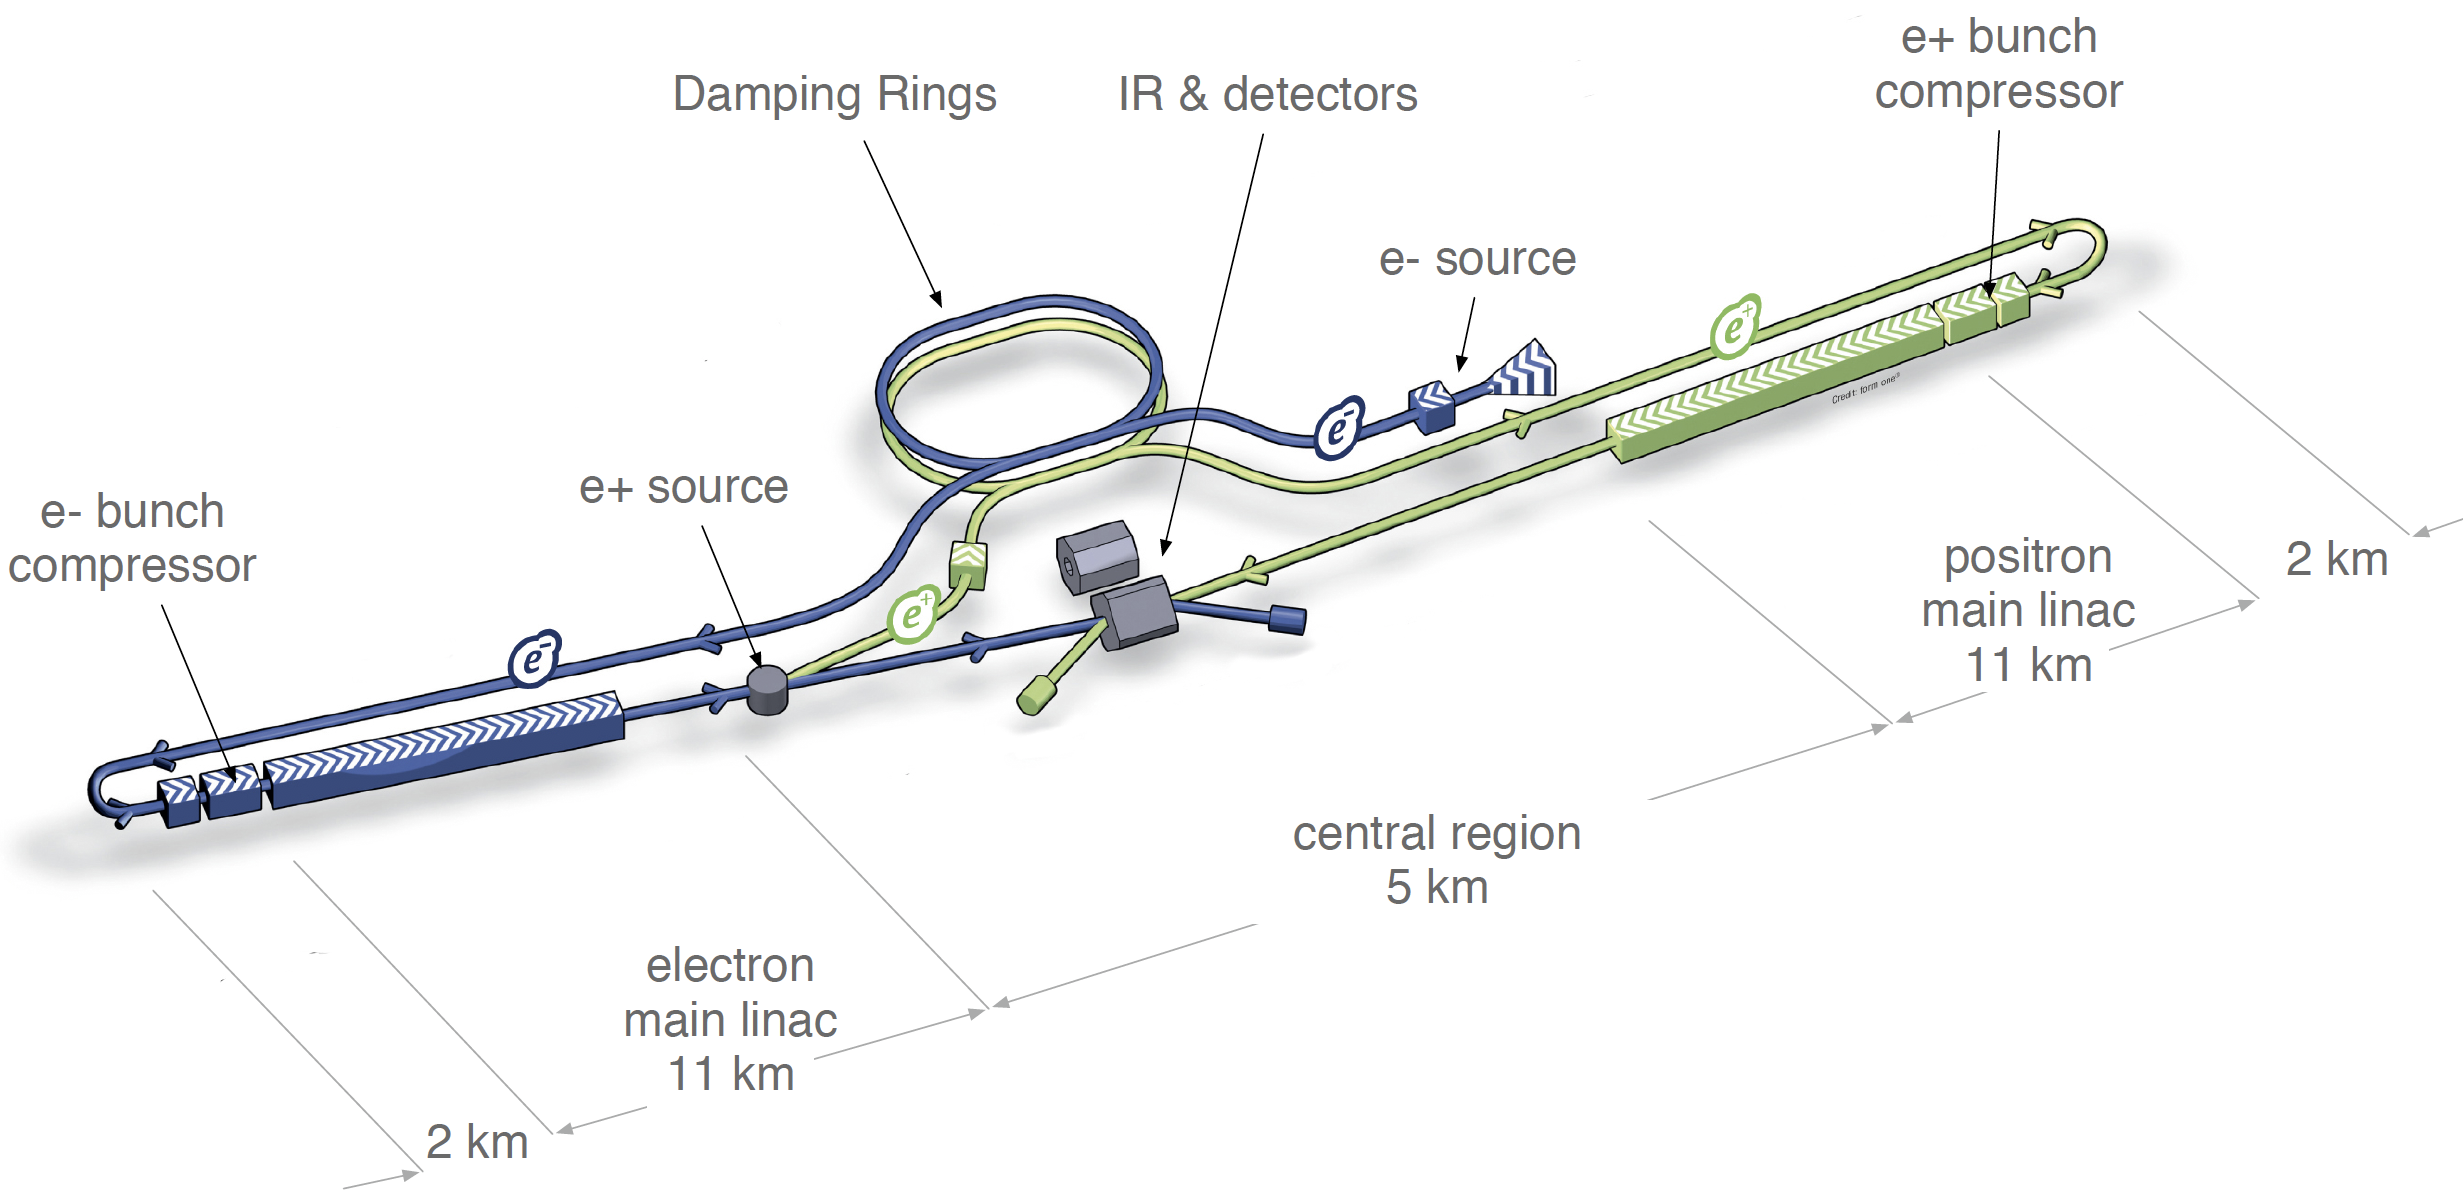
\includegraphics[width=140mm, keepaspectratio]{pictures/ILC}
% \caption{ILC accelerator schematic layout \cite{ILC:cdr}.}
% \label{fig:ILC_schematic}

% \end{figure}






% \begin{figure}[!htb]
% \centering
% 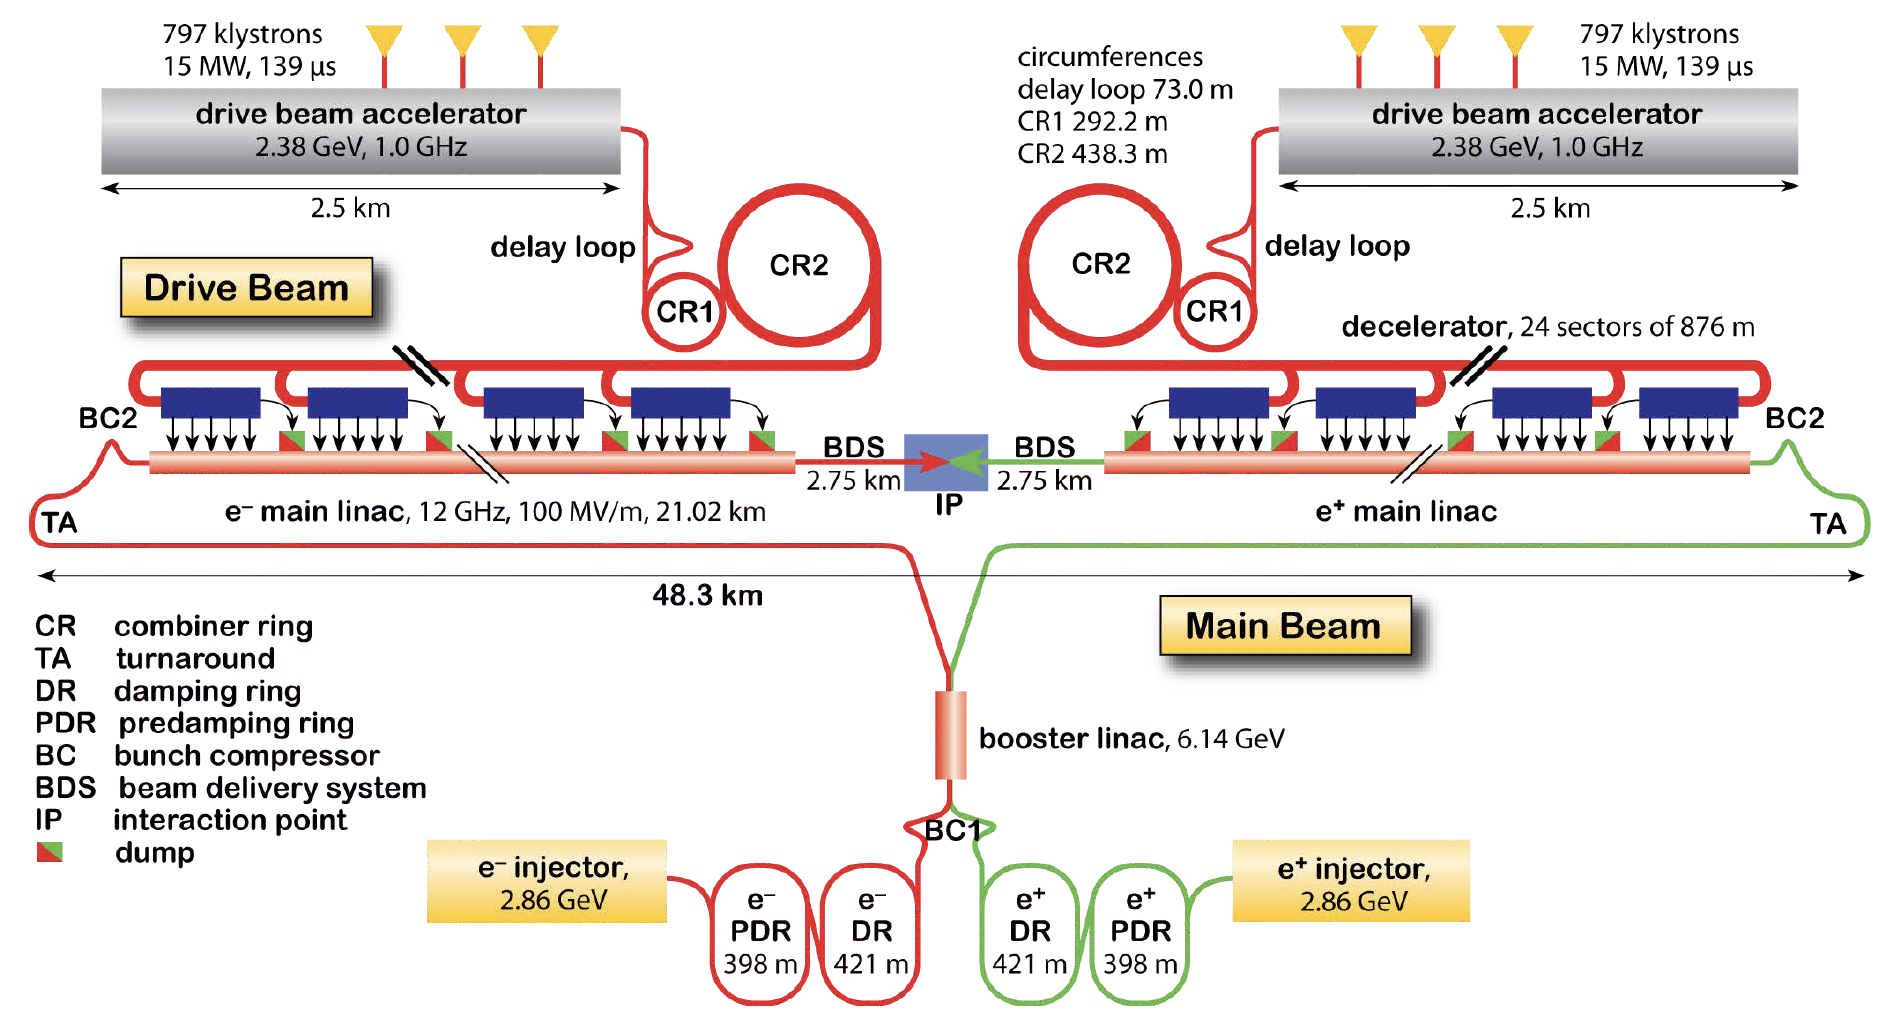
\includegraphics[width=140mm, keepaspectratio]{pictures/CLIC}
% \caption{CLIC accelerator schematic layout \cite{CLIC:cdr}.}
% \label{fig:CLIC_schematic}

% % \vspace{3mm}



% \end{figure}


\begin{figure}[!h]
\centering
\vspace{10mm}
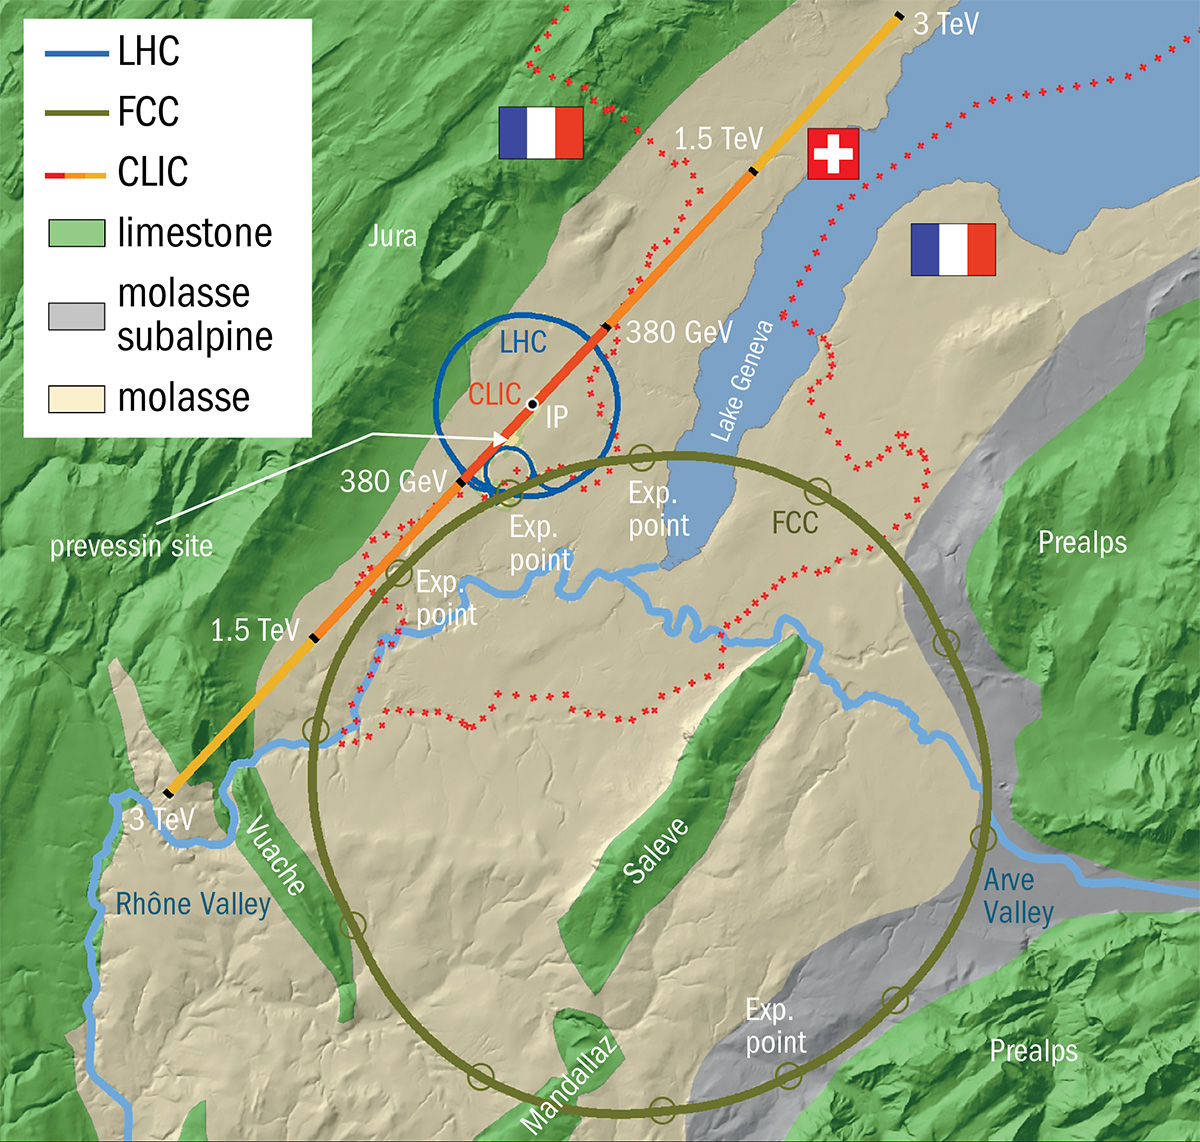
\includegraphics[width=120mm, keepaspectratio]{pictures/FCC_vs_CLIC_vs_LHC}
\caption{Dimension comparison of the CLIC and FCC project with the existing LHC accelerator in the Geneva area \cite{CERN-COURIER-59-5}.}
\label{fig:FCC_vs_LHC}
\end{figure}

\begin{figure}[!h]
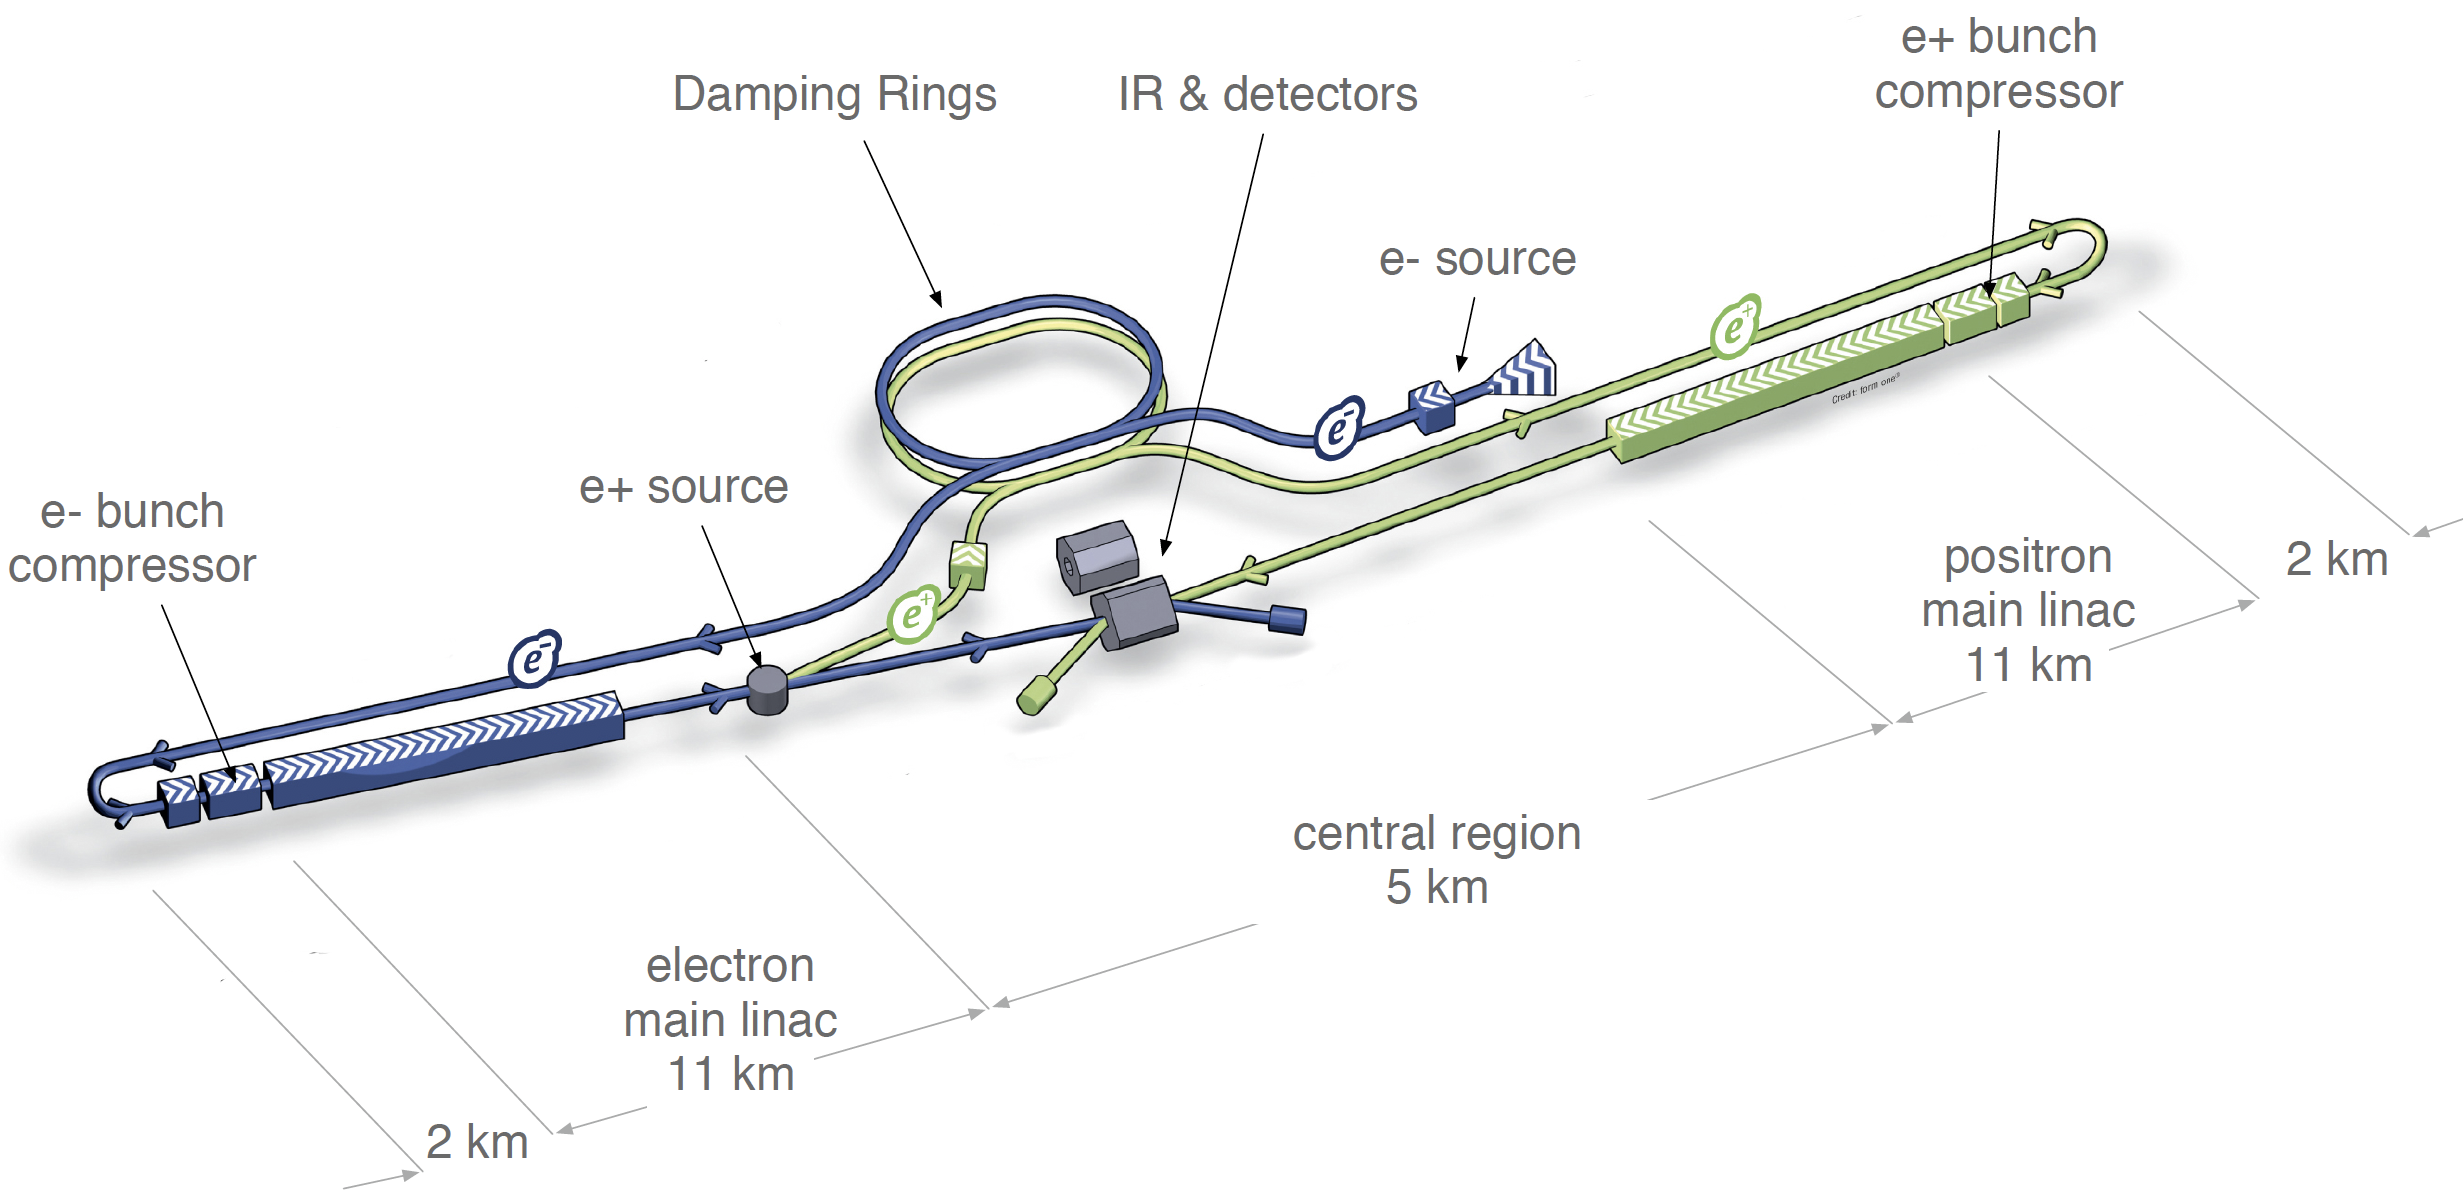
\includegraphics[width=140mm, keepaspectratio]{pictures/ILC}
\caption{ILC accelerator schematic layout \cite{ILC:cdr}.}
\label{fig:ILC_schematic}

\vspace{5mm}
\centering
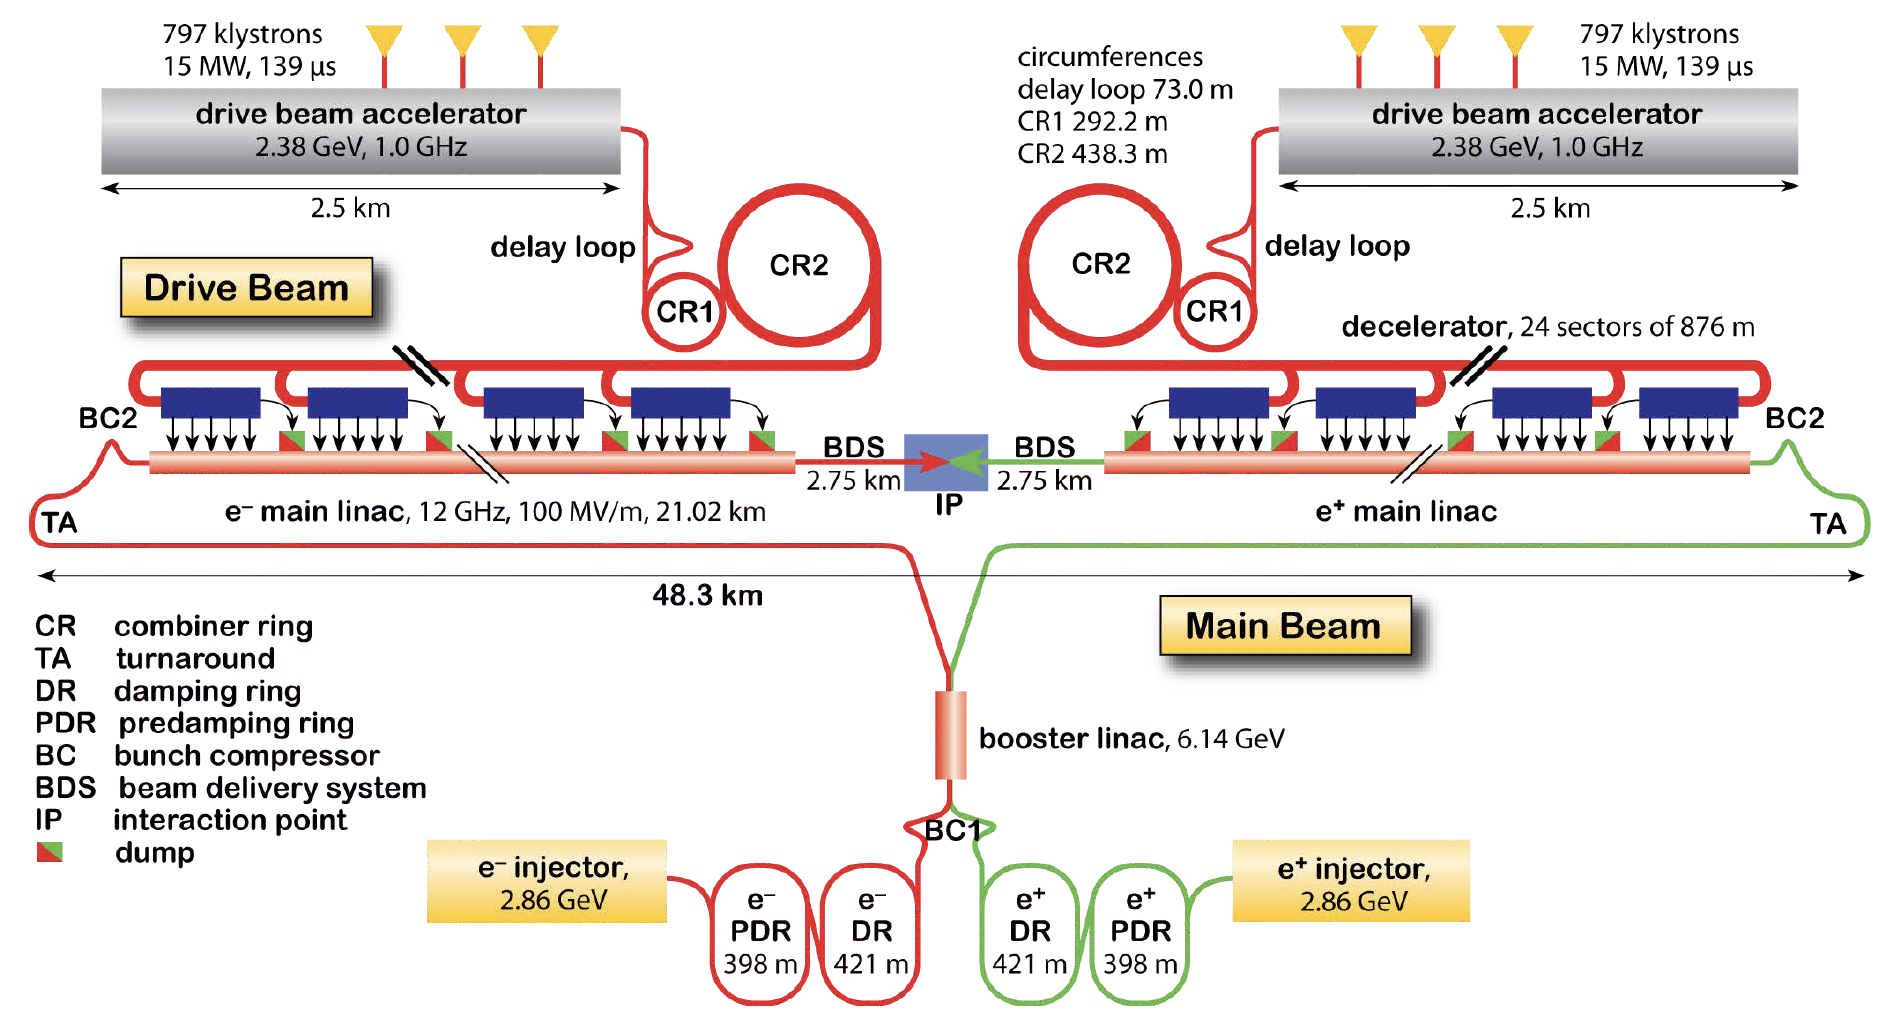
\includegraphics[width=140mm, keepaspectratio]{pictures/CLIC}
\caption{CLIC accelerator schematic layout \cite{CLIC:cdr}.}
\label{fig:CLIC_schematic}

% \vspace{3mm}



\end{figure}


\newpage
\section[Two-beam acceleration technologies]{Two-beam acceleration technologies}\label{sec:two_beam_tech}

RF cavities have been the workhorse of modern accelerators. The RF power is traditionally produced starting from an electrical signal and amplified, usually in the final stage with klystrons. Then it is injected into resonant cavities with an appropriate phase to accelerate the beam once it passes through the cavity \cite{Wangler:book}. The use of RF-based technology is ultimately limited by breakdowns, due to the high surface electric field in the equipment \cite{KilpLimit}. In recent years, in an attempt to improve performance and energy efficiency, novel techniques have been studied to supply fast pulses of high power to the beam. Their common denominator is abandoning the conventional RF production and instead feeding accelerating structures with energy extracted from another beam. The new schemes work like an electrical transformer, where a `drive', high power, beam is depleted of energy, that is transferred to a `witness' beam that is accelerated. An advantage of this approach is the possibility to store a large amount of energy in the drive beam before eventually transferring it to the witness. The drive beam can be either a photon beam (i.e. a high power laser) or a charged particle beam. 

The two-beam acceleration concept for a linear collider was already proposed in the past by the CLIC study \cite{HOPKINS198415} with the drive beam power extracted in the form of RF and transferred to a second parallel accelerator to accelerate the witness `main' beam. The proof of feasibility of two-beam acceleration has been demonstrated in the CTF3 facilty at CERN \cite{Corsini:2017use}. Nevertheless, CLIC remains limited by the breakdowns occurring in its normal-conducting accelerating cavities. This effect is limited with careful design and surface treatment to reduce the surface electric field, allowing accelerating gradients in excess of 100~MV/m to be achieved \cite{PhysRevAccelBeams.21.061001, PhysRevAccelBeams.21.102002}. 

To overcome the breakdown limitation of metals and further increase the accelerating gradients, two different approaches are being studied: dielectric accelerating structures, and acceleration in plasmas. Both work with an accelerating field frequency much higher than the typical RF, usually exceeding hundreds of GHz for dielectric structures and in the THz range for plasma acceleration. 

The proposed accelerating structures made of dielectric materials can be both particle beam driven \cite{DWA_1} and laser driven \cite{RevModPhys.86.1337}. These technologies already demonstrated accelerating gradients 2-3 times larger than the most efficient metal cavities \cite{Peralta:2013vpa} ultimately exceeding GV/m \cite{DWA_2}.

Even higher accelerating gradients are possible when using an already `broken-down' medium, e.g. plasma \cite{PhysRevLett.43.267,Chen:1984up} in a scheme known as Plasma Wakefield Acceleration (PWA), with the drive beam traversing a plasma column. The neutral plasma density is locally perturbed as the drive beam passage displaces some of the plasma electrons, generating regions with high electric field. This can be achieved by exploiting the ponderomotive force of a laser beam pulse on the plasma electrons (Laser Wakefield Acceleration, LWFA) \cite{Mangles:2004ta, Faure:2004tc} or by using the space-charge force from a relativistic particle beam (Particle Wakefield Acceleration, PWFA) \cite{Blumenfeld:2007ph, Litos:2014yqa}. This process is schematically shown in Fig.~\ref{fig:plasma-acc-scheme}, where the electron drive bunch has generated a plasma `bubble' in which the electron density is reduced. 


\begin{figure}[!t]
\centering
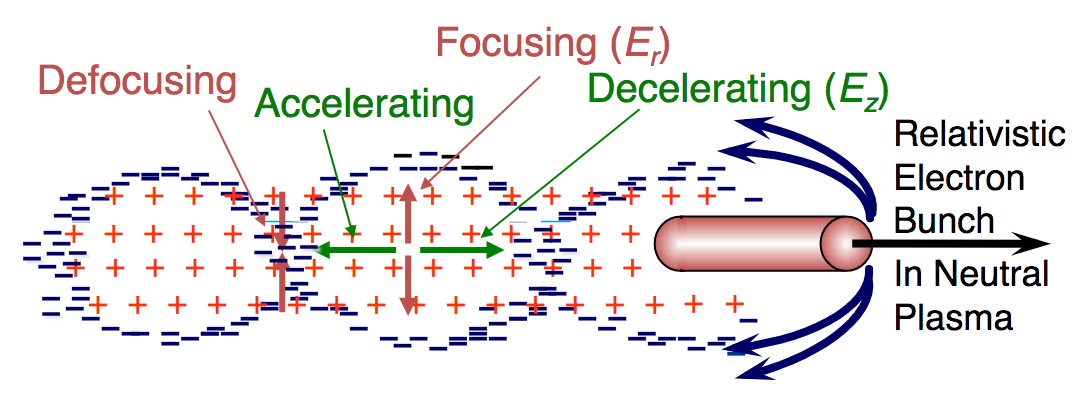
\includegraphics[width=140mm, keepaspectratio]{pictures/Plasma_schematic}
\caption{Schematic representation of the plasma wakefield formation by an electron driver bunch. Adapted from~\cite{Muggli:2203633}.}
\label{fig:plasma-acc-scheme}
\end{figure}


The plasma density perturbation depends on the drive beam intensity, resulting in different plasma wave regimes. For small driver intensities, linear plasma density waves will occur, which is known as the linear regime. Nonlinear waves of growing amplitude arise with an increasing driver intensity, up to reaching the blow-out or `bubbling' regime in which the plasma electrons trailing the driver are completely expelled from the bubble and form a sheath on the bubble edge. In order to characterise the plasma wave regime, two figures of merit are defined for LWFA and PWFA respectively:
\begin{equation}
a_0 = \frac{eE_0\lambda_0}{2\pi m_e c^2} \qquad \qquad \Lambda_0 = \frac{n_b}{n_0} k^2_p \sigma_r^2
\end{equation}
where, $a_0$ is the normalised field strength, $E_0$ and $\lambda_0$ are the laser electric field intensity and wavelength, $m_e$ is the electron mass and $c$ is the speed of light in vacuum. For PWFA, $\Lambda_0$ is the normalised beam charge per unit length \cite{limits_plasma_acceleration}, $n_b$ and $n_0$ are the driver bunch and plasma densities, $\sigma_r$ is the driver transverse size and $k_p$ is the plasma wave number. The latter is given by the relation $k_p = w_p/c$, where the plasma frequency is defined as $\omega_p = \sqrt{\frac{n_0e^2}{m_e\epsilon_0}}$ and $\epsilon_0$ is the vacuum permittivity. The linear regime occurs when the normalised intensity $a_0$ or $\Lambda_0$ are less than 1 (ideally $\ll 1$).  

An analytical description of the electric field can be derived for a 3D non-relativistic plasma in the the linear regime~\cite{Ruth:1986pqa}. The longitudinal and transverse electric field are given by:
\begin{equation}
E_z \simeq -A\left(1-\frac{r^2}{a^2} \right) \, cos\left(k_pz-\omega_pt\right) \, , \qquad r \ll a \label{eq:e_long}
\end{equation}
\begin{equation}
E_r \simeq 2A\left( \frac{r}{k_pa^2} \right) \, sin\left(k_pz-\omega_pt\right)  \, , \qquad r\ll a \label{eq:e_trans}
\end{equation}
where $r$ and $z$ are the radial and longitudinal coordinates, $a$ is the driver radius, $\omega_p$ and $k_p$ are the plasma frequency and wave number and $t$ is the time variable. These expressions hold under the assumptions that $k_pa \gg 1$ and $r \ll a$. The $A$ factor is defined for LWFA and PWFA as
\begin{equation}
A_\text{LWFA} = \frac{\omega_p r k_p e E_0^2}{8 \omega^2 m_e}
\quad,\quad \qquad
A_\text{PWFA} = \frac{8eN}{a^2}
\end{equation}
where $N$ is the number of particles in the PWFA driver, $\omega$ is the laser frequency and $E_0$ is the laser electrical field. 
Equations \ref{eq:e_long} and \ref{eq:e_trans} show that there is a $\pi/2$ phase difference between the longitudinal (accelerating or decelerating) and the transverse (focusing or defocusing) electric fields. Therefore, only one quarter of the wake period can be used to accelerate the witness beam while simultaneously focusing it, as shown in Fig.~\ref{fig:plasma_focusing}. 

An electron beam injected into a proper region of the plasma bubble will be therefore accelerated and focused respectively by the longitudinal and transverse electric field. Acceleration of externally-injected electron beams has been experimentally achieved driven by both electron \cite{Litos:2014yqa} and proton beams \cite{Adli:2018end}.

\begin{figure}[!b]
\centering
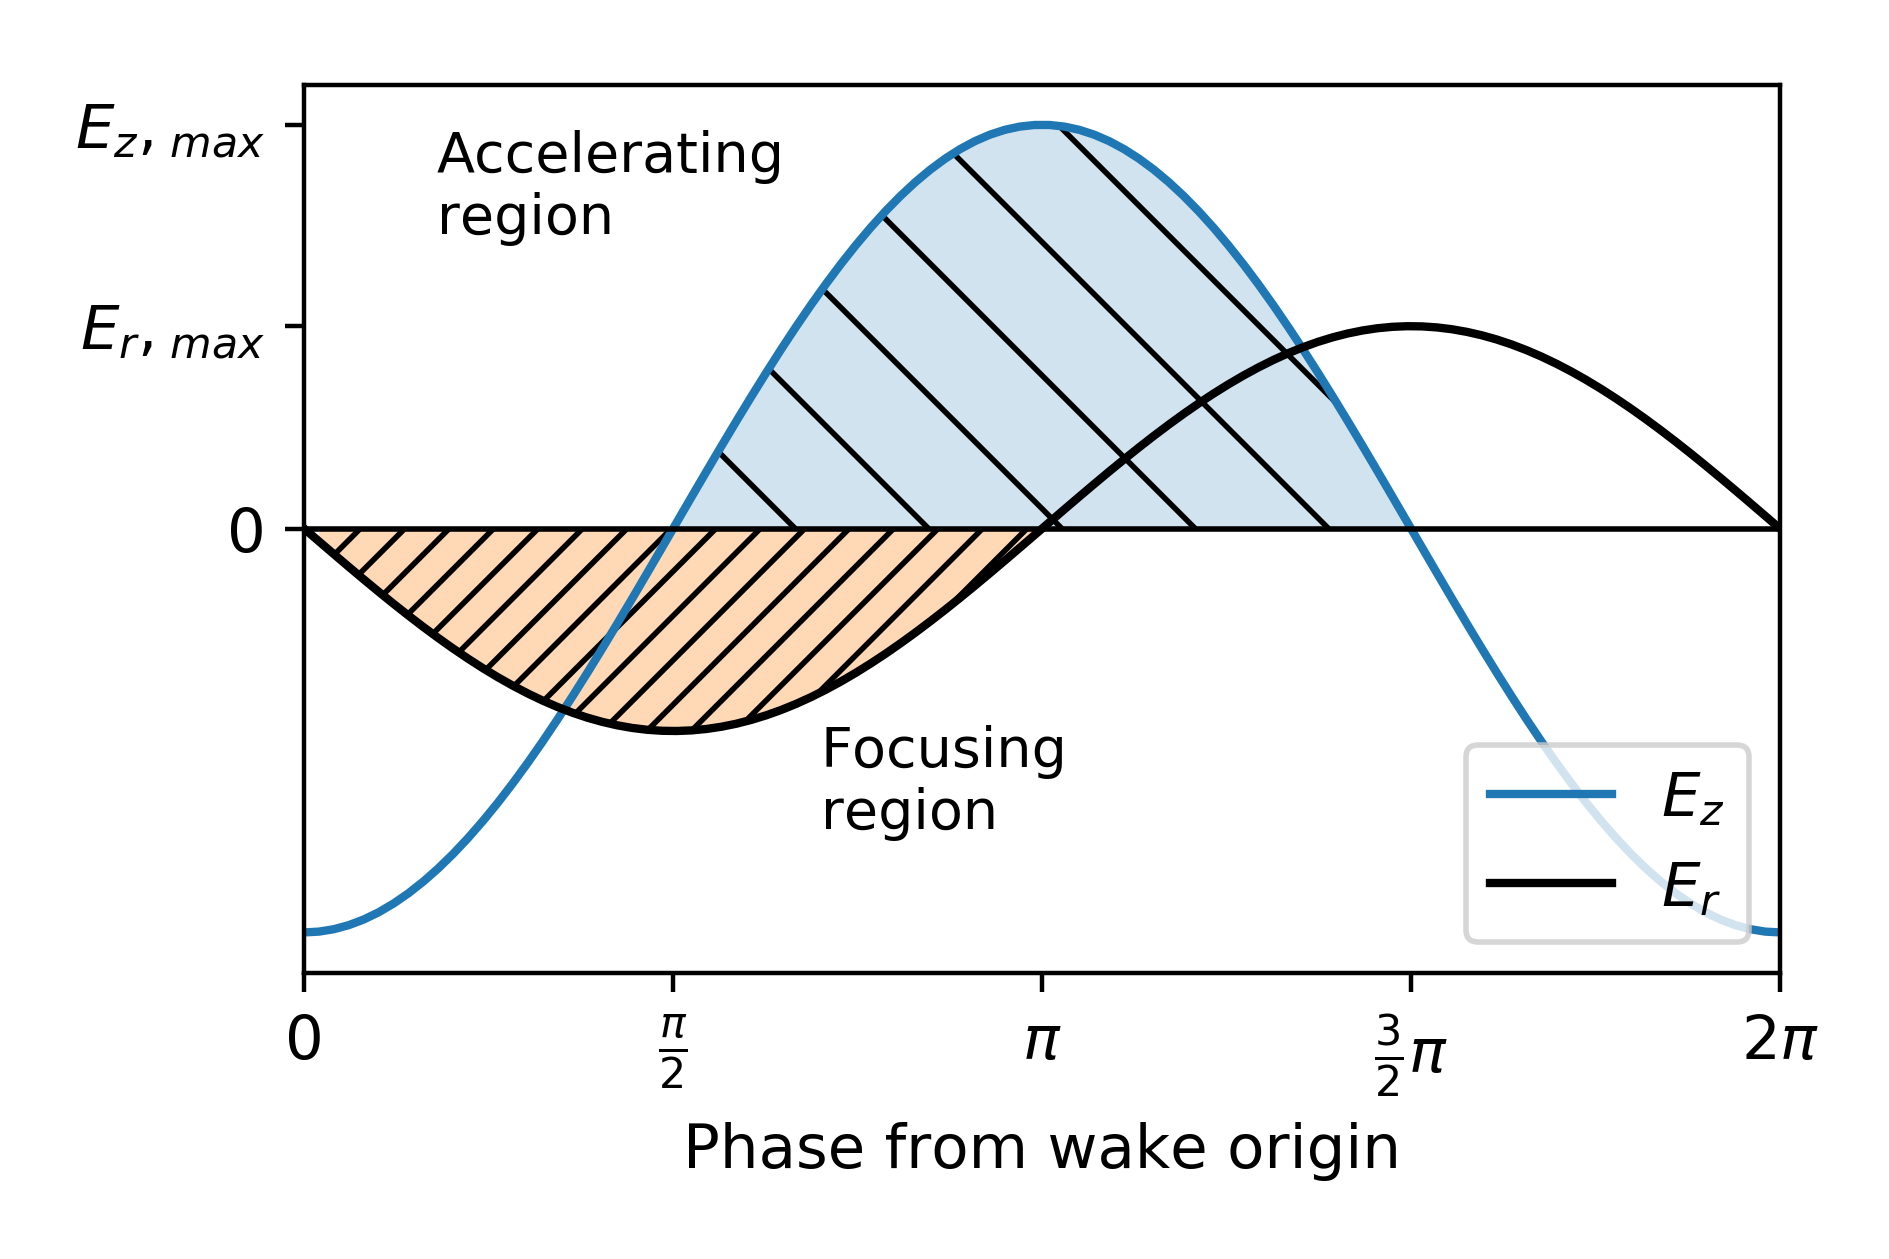
\includegraphics[scale=0.8, keepaspectratio]{pictures/Plasma_focusing_theory}
\caption{The longitudinal and radial electric fields in a plasma bubble from the approximated solutions for linear waves in a 3D plasma. Only one quarter of the phase is useful for accelerating a particle beam without increasing its transverse size. }
\label{fig:plasma_focusing}
\end{figure}


The maximum achievable accelerating gradient in a plasma accelerator is given by the cold nonrelativistic wavebreaking field  
\begin{equation}
E_z = \frac{m_e c^2}{\epsilon_0} \sqrt{n_e} \approx 96 \sqrt{n_0}\label{eq:gradient_max}
\end{equation}
where $n_0$ is the plasma density in $\mathrm{cm}^{-3}$ \cite{Chen:1984up, RevModPhys.81.1229}. As plasma densities of the order of $10^{18} \text{ cm}^{-3}$ are achievable,  accelerating gradients of 100's~GV/m become within reach \cite{Blumenfeld:2007ph, Malka1596}, three orders of magnitude higher than the best RF cavities. 

Plasma wakefield acceleration is particularly challenging not only due to the inherent complexity of the setup, but also because of the stringent beam parameters required. In fact, the bunch length $\sigma_z$ \cite{limits_plasma_acceleration} and the transverse size $\sigma_r$~\cite{PhysRevLett.109.185007} must satisfy the following conditions to efficiently drive plasma wakefields while avoiding development of any instabilities:
\begin{equation}
k_p\sigma_z\sim\sqrt{2}\label{eq:lim_long}
\end{equation}
\begin{equation}
k_p\sigma_r\sim1\label{eq:lim_trans}
\end{equation}
Considering a plasma density between $10^{14}$ and $10^{18}$~cm$^{-3}$, these conditions translate to a required transverse size range between 0.75~mm and 7.5~$\mu$m, respectively, and a bunch length between 0.5~mm and 5~$\mu$m. As high plasma densities are desirable due to the higher achievable accelerating gradient (see Equation~\ref{eq:gradient_max}), one can see how challenging beam focusing is and the required beam positioning accuracy needed for these experiments. 









\section[The AWAKE experiment]{The AWAKE experiment}

The Advanced Wakefield Experiment (AWAKE) at CERN studies plasma wakefield acceleration driven by a high energy proton beam, and demonstrated acceleration of an electron bunch in 2018 \cite{Adli:2018end}. To achieve acceleration, a proton drive bunch is merged in a common beamline with a laser beam and an electron bunch \cite{Bracco:1965994}. They then propagate to a plasma cell, where the PWFA takes place. The experiment layout is presented in Fig.~\ref{fig:awake_layout}.

The 400~GeV proton driver bunch is produced in the CERN accelerator chain, shown in Fig.~\ref{fig:cern_injectors}. The proton beam is initially produced in Linac~2 and accelerated up to an energy of 50~MeV. The beam is then transferred to the Proton Synchtron Booster (PSB), and it is accelerated up to 1.4~GeV. At this point, it is extracted to the Proton Synchrotron (PS), and once the energy of 26~GeV is reached, the beam is sent to the Super Proton Synchrotron (SPS). In the SPS the beam is accelerated to 400~GeV. It is then extracted through the CNGS extraction line, that reaches the AWAKE experiment after $\sim 1$~km \cite{Elsener:530678}. Currently, a substantial upgrade of the CERN injector chain is being realised \cite{LIU}, affecting mostly Linac 2, PSB and PS. This upgrade does not impact the AWAKE proton beam production, as no modification in the proton beam parameters is expected at the moment. The proton bunch has a bunch length of 6-12~cm, with a bunch population that can be selected in the range $1-3\times10^{11}$ protons per bunch (ppb), and it is focused down to an r.m.s. transverse size of $\sim 200\,\mu$m at the plasma cell entrance \cite{Adli:2018end}. 

\begin{figure}[!bh]
\centering
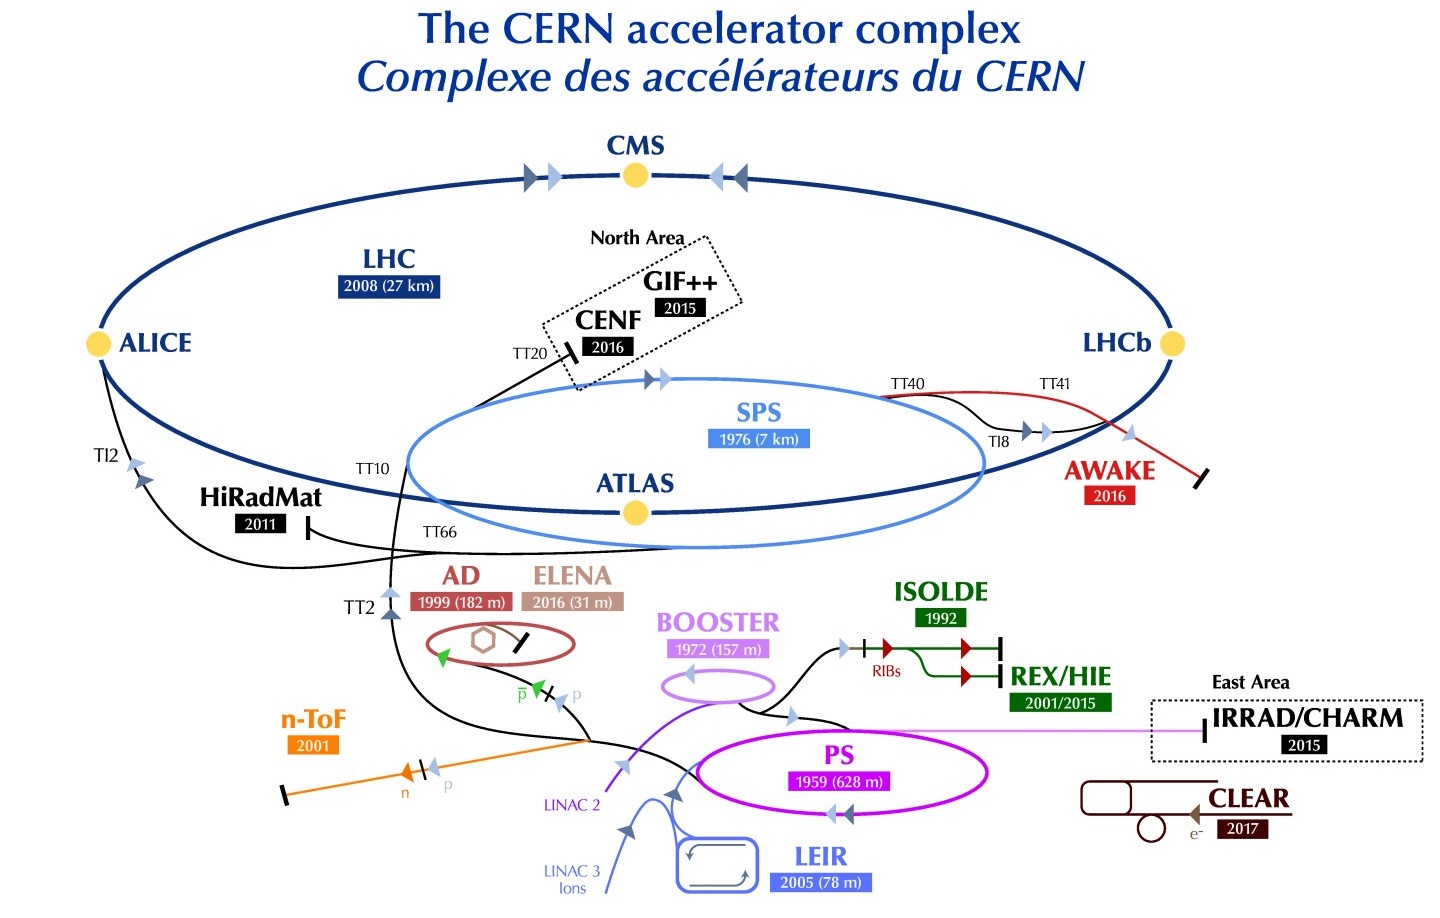
\includegraphics[width=14cm, keepaspectratio]{pictures/cern_complex}
\caption{The CERN accelerator complex layout. The AWAKE proton beam is produced in the SPS (light blue ring in the centre) and extracted through the CNGS transfer line (drawn in red) to the AWAKE experiment. Adapted from  \cite{cern_acc_complex_layout}.}
\label{fig:cern_injectors}
\end{figure}

\begin{landscape}
\begin{figure}
\centering
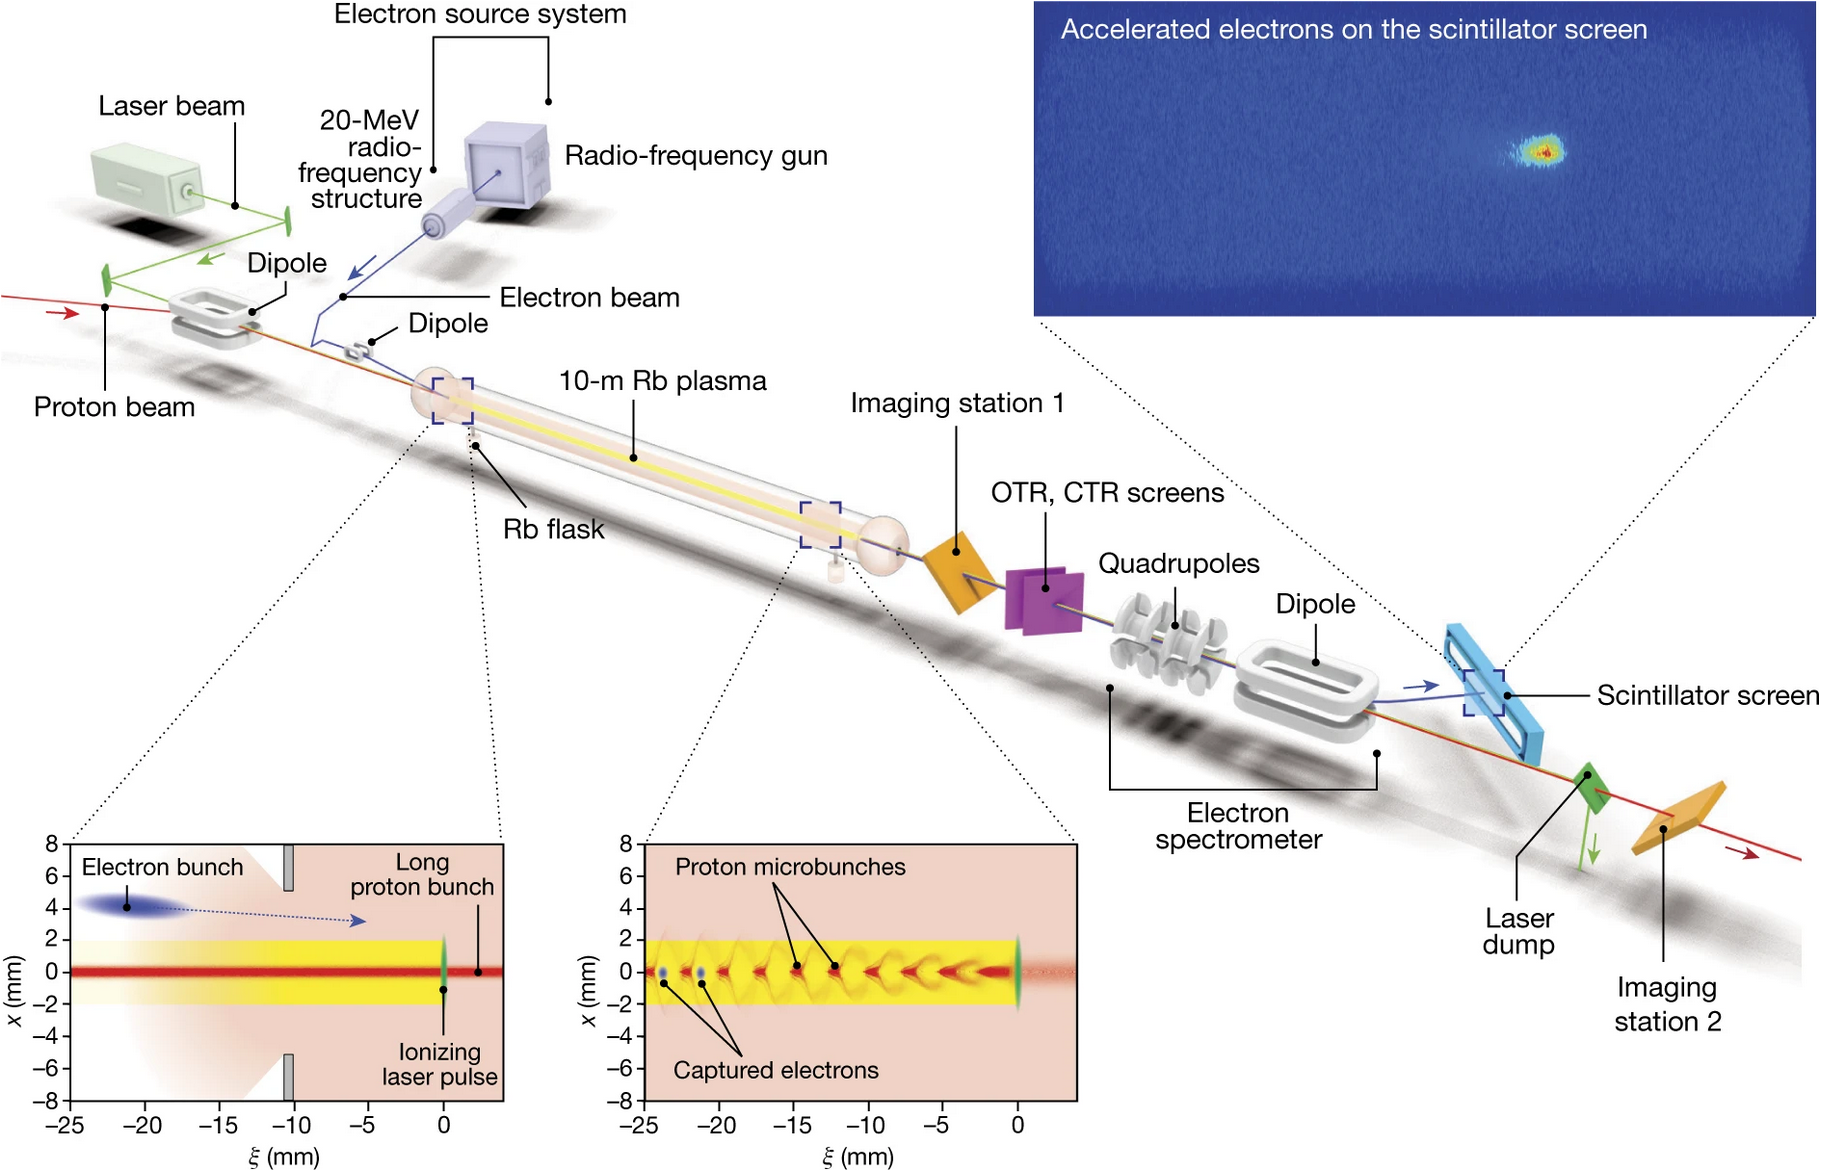
\includegraphics[width=18cm, keepaspectratio]{pictures/awake_layout}
\caption{Layout of the AWAKE experiment \cite{Adli:2018end}. The bottom left plot shows the laser, proton and electron beam at the plasma cell entrance. The adjacent plot shows the laser beam, the self-modulated proton beam and the electron beam captured by the generated wakefields. The top plot shows an example of the spectrometer images.}
\label{fig:awake_layout}
\end{figure}
\end{landscape}





The laser beam is used to ionise the rubidium (Rb) gas present in the plasma cell, resulting in the formation of a plasma column. AWAKE uses a 120~fs-long laser pulse with a wavelength of 780~nm and pulse power up to 450~mJ \cite{Fedosseev:2016ccm}. The laser beam is transversely focused to 1~mm (full-width at half-maximum, FWHM) inside the plasma cell.

The electron witness beam is produced in a dedicated photoinjector close to the experiment. Its energy can be selected in the range of $10-20$~MeV with a $0.1-1$~nC charge and a bunch length of $1-4$~ps $(1\sigma)$ \cite{Pepitone:2018gwl, Kim:2706086}.

The plasma cell is 10~m long and has a 4~cm diameter. Two rubidium flasks are installed at each end and the Rb gas density is controlled in the range $10^{14}-10^{15}$~cm$^{-3}$ by adjusting the cell temperature \cite{Plyushchev:2017kqg}.




To successfully drive wakefields to accelerate electrons, a proton bunch shorter than that produced in the SPS is necessary. In fact, directly using the SPS proton beam as a driver would require the use of a low plasma density, that results in a modest accelerating gradient below 10~MV/m \cite{patric_AAC_seminar}. To overcome this problem, the experiment works in two steps: in the first part of the plasma cell, the proton bunch is fragmented into a train of shorter bunches by a process called Seeded Self Modulation (SSM) \cite{phys_self_modulation}. For a relativistic proton bunch \cite{PhysRevLett.104.255003} it is achieved by co-linear steering of the laser pulse and the proton bunch (see the inset in the bottom left of Fig.~\ref{fig:awake_layout}). The laser ionises the Rb vapour into plasma by creating a sharp ionisation front. The transverse wakefields induced in the plasma determine a periodic focusing and defocusing of the proton beam, where the period length is determined by the plasma parameters. The protons in the defocusing regions are consequently expelled, transforming the proton bunch in a train of micro-bunches serpared by one plasma wavelength (see the inset in the center bottom of Fig.~\ref{fig:awake_layout}). The micro-bunch train resonantly drives large amplitude wakefields in the plasma. The modulation of the proton bunch into more than 20 micro-bunches has been demonstrated at AWAKE \cite{PhysRevLett.122.054802}. The electron bunch is then inserted into the appropriate point in the train of micro-bunches and accelerated. It does not participate in the SSM process, as it is injected with a spatial offset and a temporal delay. The electron and proton beams are overlapped a few metres downstream from the plasma cell entrance, after the SSM process has taken place. The generated wakefields are suitable to accelerate the electron beam if it is placed at the correct longitudinal position in the wakefields. Selection of the relative delay between the beams and the beam trajectories is crucial for achieving acceleration. Boosting electrons from 18.8~MeV up to an energy of 2~GeV in a 10~m plasma cell has been demonstrated~\cite{Adli:2018end}.






\subsection[Particle-beam instrumentation for AWAKE]{Particle-beam instrumentation for AWAKE}\label{sec:AWAKE_instrumentation}

Given the remarkable complexity of the AWAKE facility, a large amount of particle-beam instrumentation is necessary to operate and diagnose the multiple beamlines. Various measurements are performed on the beams, including electron and proton beam positions, transverse profiles, temporal synchronisation between the beams, charge measurements, and an energy measurement of the electron beam. The systems most relevant for the work presented in this thesis are briefly described below, while a detailed description of the AWAKE particle-beam instrumentation can be found in \cite{Mazzoni:2017gek, Gorgisyan:2649943}. 

The transverse beam profile is measured with removable screens that can be inserted into the beamline. Two types of screens are used, based on   scintillation~\cite{Behrens:2012zz} and Optical Transition Radiation (OTR)~\cite{Welsch:2006bj}. Chromox scintillating screens (Al$_2$O$_3$:CrO$_2$) are used for the profile measurements due to their high light yield, but feature a long decay time (>100 ms). Silver-coated Silicon OTR screens can also be used for the beam profile measurement, but they have a more modest light yield. The advantage of OTR screens is the instantaneous emission, that is used for beam synchronisation purposes. The two types of screens offer a comparable spatial resolution. A total of six screen imaging stations are present in AWAKE, two of them in the electron beamline, two in the common beamline upstream of the plasma cell, and two in the common beamline after the plasma cell. The beam profile in the common line can be measured with a resolution of $50\mu$m.

The temporal synchronisation between the beams is measured using the OTR light emitted by one of the screens. The light is then sent through an optical line to a separate room where a streak camera with a temporal resolution of 200~fs is installed. This setup can also be used to measure the longitudinal profile of the beams. Such a measurement was performed during this thesis work, therefore the detailed description of the system is presented later in Section~\ref{sec:p_temporal_profile}.

The transverse beam position is monitored with separate systems for the proton and electron beams upstream of the plasma cell. The proton Beam Position Monitors (BPMs) are placed along the whole transfer line starting from the SPS and extend beyond the plasma cell to the proton beam dump. The system is composed of 21 sensors formed of four electrostatic buttons. Laboratory and beam-based tests showed a 40~$\mu$m resolution for high intensity beams $>10^{11}$~ppb \cite{BarrosMarin:2018yvv}. The electron BPM system is made of shorted stripline BPMs \cite{Shengli:tipp, Liu:2019ilj}. Five of them are installed in the common beamline, while seven are installed in the electron beamline. In laboratory and beam-based tests they exhibited a resolution below 10~$\mu$m.




\section{Motivation for this work}

A number of novel techniques showed both theoretically and experimentally that unprecedented accelerating gradients can be achieved. To turn these experiments into future operational accelerators, development of novel beam instrumentation and diagnostic techniques is necessary. The existing technology is challenged by two major issues: novel acceleration schemes often involve more than one beam, and they require extremely precise and accurate instruments due to small beam sizes and short pulse lengths. These problems apply not only to plasma-based accelerators, whose strict requirements on the beam size are outlined in Equations~\ref{eq:lim_long} and \ref{eq:lim_trans}, but also to more traditional designs. For example, the CLIC facility would require measurements of the transverse position of beams to the nanometre level in its final-focus system.

This thesis work contributes to the field of novel beam instrumentation for facilities using multiple particle beams. The presented research addresses the problem of detecting the position of a shorter and less intense electron witness bunch in AWAKE, when a longer and more intense proton driver bunch is co-propagating in the beam pipe. Currently, the electron BPM system is not capable of measuring the electron beam position when the proton beam is present. The developed techniques are also valid for all accelerators that use short bunches, of the order of ps-long or shorter, e.g. Free Electron Lasers (FELs).
